\documentclass[12pt]{article}
\usepackage{frExamplee}
\usepackage{booktabs}       % professional-quality tables
\usepackage{amsfonts}       % blackboard math symbols
\usepackage{amsmath}
\usepackage{enumitem}
\usepackage{listings}
\lstset{
    language=Python,
    basicstyle=\scriptsize\ttfamily,
    keywordstyle=\color{blue},
    commentstyle=\color{green!50!black},
    stringstyle=\color{red},
    showstringspaces=false,
    numbers=left,
    numberstyle=\footnotesize,
    numbersep=5pt,
    frame=single,
    breaklines=true,
    breakatwhitespace=true,
    tabsize=4,
    captionpos=b
}
\usepackage{amssymb}
\usepackage{graphicx}
\usepackage{csquotes}
\usepackage[backend=biber, style=ieee,]{biblatex}
\usepackage{setspace}
\usepackage[usenames, dvipsnames]{xcolor}
\usepackage{xspace}
\usepackage{caption}
\usepackage{subcaption}
\usepackage{multirow}
\usepackage{float}
\usepackage{wrapfig}
\usepackage{placeins}
\usepackage{algpseudocode}
\usepackage{algorithm}
\usepackage{algorithmicx}
\usepackage{hyperref}
\usepackage{setspace}
\usepackage{fancyhdr} 
\fancyhf{}
\cfoot{\thepage}
\pagestyle{fancy}
\renewcommand{\headrulewidth}{0pt}%

\addbibresource{FRtemplates/frExampleRefs.bib}
\title{Recreating the Franck-Hertz Experiment}
\author{
Tony Wang \href{https://orcid.org/0009-0009-3015-7192}{
\includegraphics[height=12pt]{figure/orcid.png}}\\
\texttt{1009027447 | wangq330} \\
\texttt{tonyivt.wang@mail.utoronto.ca}\\
\And
Natasha Yang \href{https://orcid.org/12345}{
\includegraphics[height=12pt]{figure/orcid.png}}\\
\texttt{1008975575 | yangx315} \\
\texttt{nxy.yang@mail.utoronto.ca} \\
\And
Sharn Singh \href{https://orcid.org/12345}{
\includegraphics[height=12pt]{figure/orcid.png}}\\
\texttt{1009134492 | singh947} \\
\texttt{sharn.singh@mail.utoronto.ca} \\
}
\begin{document}
\maketitle
\begin{abstract}
In this experiment, the quantum properties of the mercury atom are investigated using the Franck Hertz experiment. By bombarding mercury atoms with a beam of electrons and observing dips in the current-voltage graph, we determined the amount of energy transferred to a Hg atom in an inelastic collision to be $\Delta E = 4.898 \pm 0.021 \rm eV$. We also found the wavelength of the photon emitted by Hg atoms when decaying from the first excited state to the ground state to be $\lambda = 275.7 \pm 7.1 \rm nm$. These values lie within $4.88\%$ of their literature values, indicating the validity of this experiment while also leaving room for improvement \autocite{hanne1988}.
\end{abstract}

%------------------------------------------------------
% 7.41 * 10^-7 [m^2/s]
\section{Introduction}
Originally performed in 1914, the Franck Hertz experiment offered compelling evidence against classical mechanics. By bombarding mercury atoms with an electron beam in an evacuated tube, James Franck and Gustav Hertz observed evenly spaced dips in the current. These dips represent discrete energy transfers from electrons to atoms during collisions, serving as a crucial experimental basis for the quantization of states \autocite{manuall}.

In this lab, we replicate the Franck Hertz experiment to illustrate the quantum nature of atoms. To achieve this, we used an evacuated tube containing an electron-emitting filament, grids for electrons to accelerate at the desired energy, an anode at which the electrons will be collected, and vaporized mercury atoms. 

We accelerate the electrons from the cathode to the collector electrode by applying a \enquote{sweeping voltage}, which linearly increases with time. As electrons travel across the evacuated tube, they collide inelastically with Hg atoms, which results in internal energy changes in the atoms. When the threshold of exciting the first energy level is reached, electrons will transfer their energy to atoms, resulting in a lower kinetic energy. As they are captured at the grid, a smaller current is observed at the collector electrode. When the threshold of exciting the next energy level is reached, a further dip in the current will be observed. At large accelerating voltages, electrons will pass through the grid and arrive at the collector electrode. In other cases. As such, when increasing the voltage applied between two electrodes, we expect to observe equally spaced current dips superimposed on a monotonically rising curve\autocite{franckhertz_mit}. The dips represent the energy transitions in the Hg atoms excited by electrons. Additionally, due to the thermionic distribution of electron velocity, we expect the dips to be not perfectly sharp\autocite{franckhertz_mit}. Rather, the lowest points in the dips represent the voltage at which the largest number of inelastic collisions occurred.

Since the energy absorbed by Hg atoms is equal to the energy used to accelerate the electron across a certain voltage, it can be represented by
\begin{equation}
    \Delta E = q \Delta V,
    \label{eq:electrical_energy}
\end{equation}
where $q$ is charge and $V$ denotes the voltage where dips occur. Additionally, since $\Delta E=\frac{hc}{\lambda}$, we have
\begin{equation}
    \lambda = \frac{hc}{q\Delta V}.
    \label{eq:Franck}
\end{equation}
where $h,c$ are Planck's constant and the speed of light, respectively.

\section{Experiment}
\subsection{Equipment and Uncertainties}
\begin{itemize}
  \item Franck-Hertz tube 
  \item Power supplies (E1, E2, E3, E4)
  \item Oven
  \item Thermometer
  \item Electrometer ($\pm 0.001{\rm A}$)
  \item Voltmeter ($\pm 0.001{\rm V}$)
  \item Computer (if used for data acquisition)
\end{itemize}

\subsection{Apparatus}
\begin{figure}[h!]
    \centering
    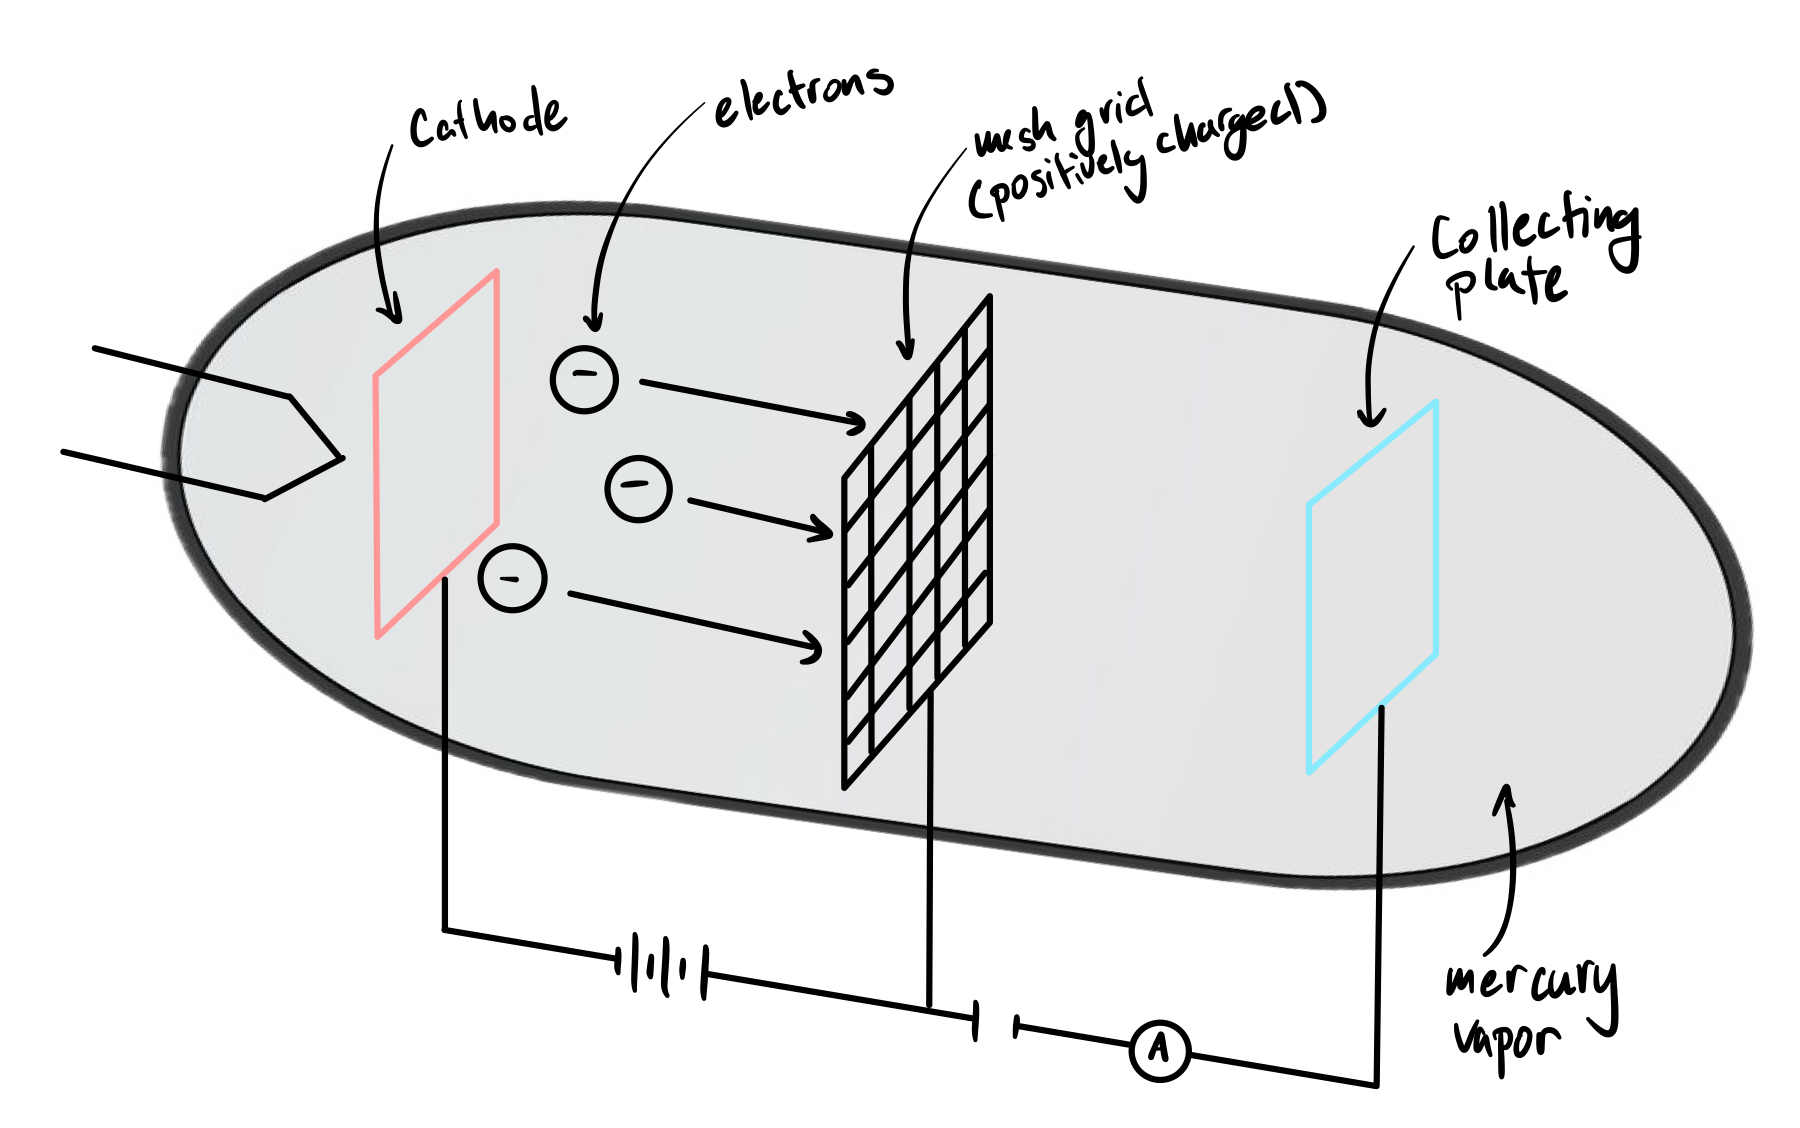
\includegraphics[width=0.7\textwidth]{figure/apparatus image.jpeg}
    \caption{Abstract sketch of the essential apparatus (Franck-Hertz Tube, E1).}
    \label{fig:1}
\end{figure}

\begin{figure}[h!]
    \centering
    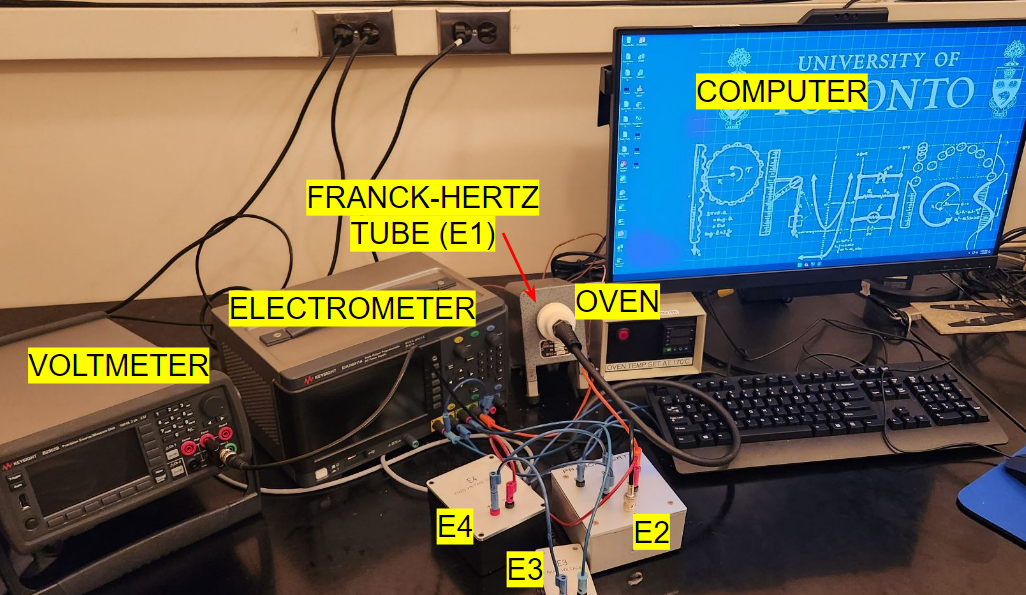
\includegraphics[width=0.7\textwidth]{figure/image of lab.PNG}
    \caption{Experimental apparatus with equipment labeled.}
    \label{fig:2}
\end{figure}

\newpage

\subsection{Method} 

\subsubsection{Preparation}
\begin{enumerate}
    \item Ensure that all equipment is set up correctly, and all components are connected (refer to Fig. \ref{fig:2}).
    \item Turn the oven on to heat the Franck-Hertz tube to the specified operating temperature, 170°C. Monitor the thermometer to ensure the temperature stabilizes. Do not let the temperature exceed 210°C. 
    \item Turn on all the power supplies (E1, E2, E3, E4). Activate the filament supply (E1) first, then E2 and E3. Make sure not to exceed the maximum voltage ratings for any component \autocite{manuall}.
\end{enumerate}

\subsubsection{Experimentation}
\begin{enumerate}
    \item  Connect the E3 voltage to the manual panel ports. Adjust E1 and E2 to achieve optimal electron emission and grid bias. 
    \item Slowly sweep the accelerating voltage (E3) from zero. Observe the electrometer reading.
    \item Look for regular rises and drops in the electrometer current. These indicate energy level transitions within the mercury atoms.
    \item If the expected fluctuations are not observed, perform the following:
    \begin{itemize}
        \item Check that all power supplies are connected.
        \item Slightly adjust the oven temperature.
    \end{itemize} 
    \item Use the computer software to collect data. Open the software.
    \item If the software has collected previous data, click \enquote{Clear Graph}. Then press \enquote{Run} to begin the voltage sweep.
    \item Once the sweep is completed, press the \enquote{Stop} button. Save the date and press \enquote{Reset} to record the next trial \autocite{manuall}. 
\end{enumerate}

\subsubsection{Data Processing}
Numerous challenges exist when post-processing data. Namely, it is difficult to precisely model the behavior of the data with a specific mathematical curve and fit it linearly. While it is completely possible to model the data with a high-term Fourier series, that would replicate every feature of the data: even the noise. Hence, we need to look back at the motivation behind this experiment and examine the purpose of fitting a curve in the first place: Finding the locations of peaks.

Since we only care about individual peaks, we can simplify the problem by slicing the data into them. By specifying the start and end limits of each peak or trough, we can fit a quadratic curve linearly to each of the intervals of interest to more accurately determine the extrema with the noise that exists. Nevertheless, finding the intervals manually is quite laborious and this process can be automated. We can simply find all the points of inflections and use those as the limits. This can be computationally done by smoothing the curve and then numerically calculating the second derivatives. 

To examine the goodness of fit, we can calculate the $R^2$ and reduced $\chi^2$ for each individual quadratic fit, as well as plot their residuals. Although these usual signs of goodness of fit do not have any holistic meaning, they can still inform us of how accurate the locations of peaks and troughs are. 

The Python script achieving everything described can be found in the appendix.


\section{Data and Discussion}
\begin{figure}[h!]
    \centering
    \begin{subfigure}{1\textwidth}
    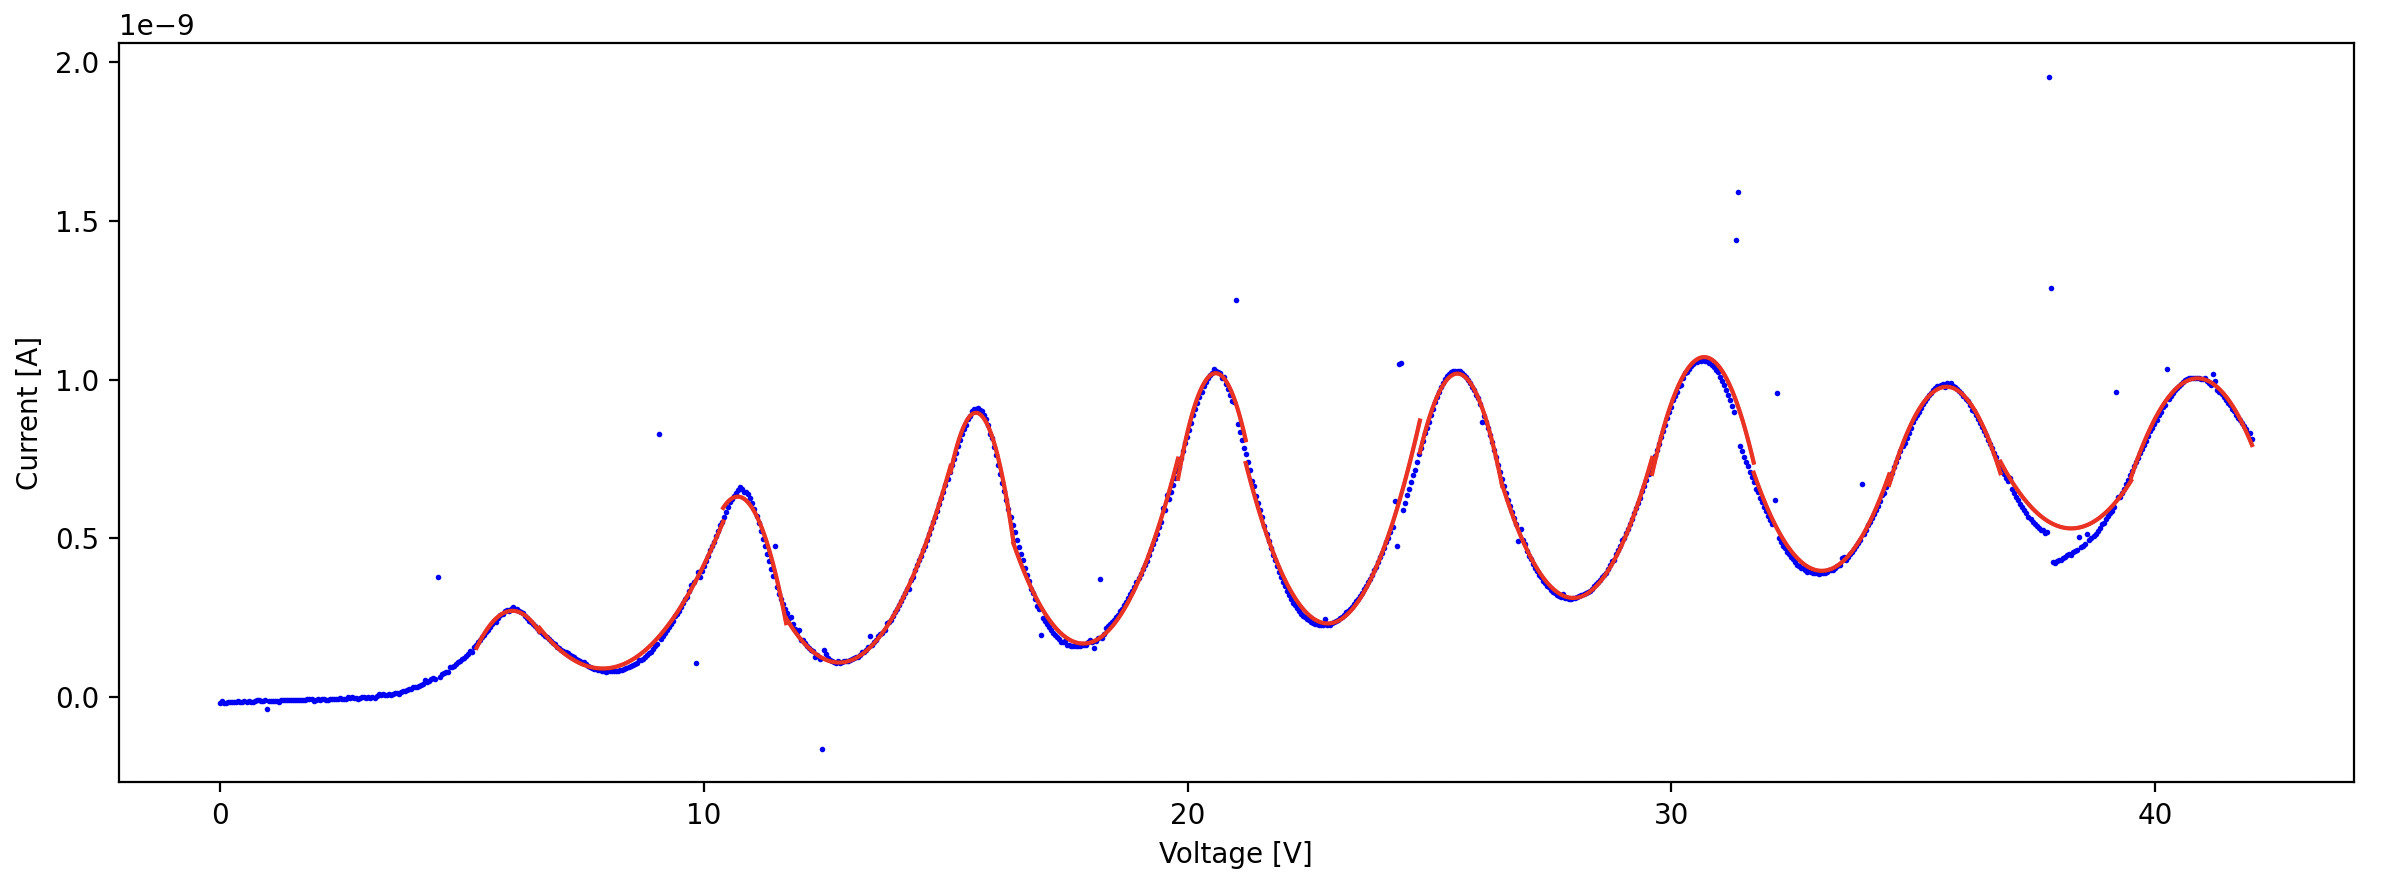
\includegraphics[width=1\textwidth]{figure/Plots/T1.png}
    \caption{\centering Sample I-V plot with each peak fitted with parabolas. Troughs are also fitted due to the nature of the plotting code, though not relevant to the analysis. The precise location of the peaks can be found in the appendix. Uncertainty bars are implemented but too little to be shown.}
        \label{fig:T4m}
    \end{subfigure}
    \begin{subfigure}{0.45\textwidth}
        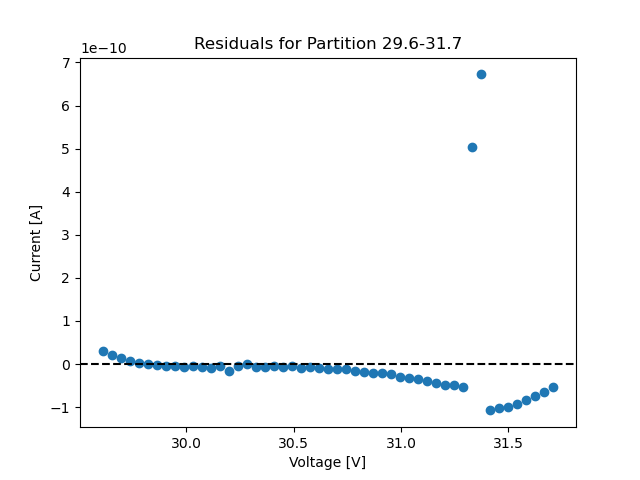
\includegraphics[width=\textwidth]{figure/Plots/11.png}
        \caption{Example residuals for a parabolic fit for data with noise}
        \label{fig:residuals1}
    \end{subfigure}
    \hfill
    \begin{subfigure}{0.45\textwidth}
        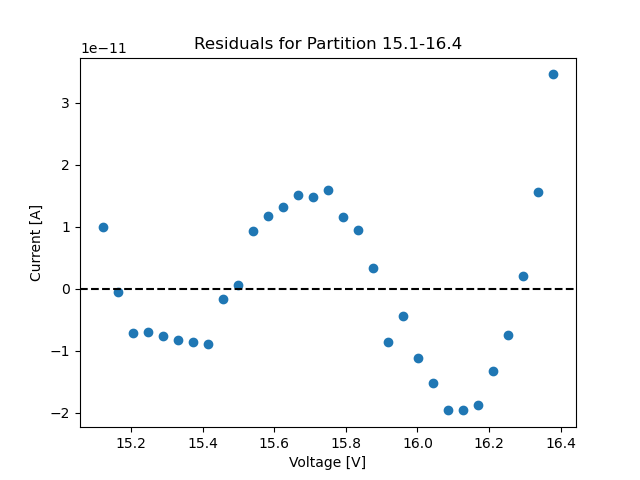
\includegraphics[width=\textwidth]{figure/Plots/5.png}
        \caption{Example residuals for a parabolic fit for part of data with minimal noise}
        \label{fig:residuals2}
    \end{subfigure}
    \caption{Example plots for data processing (Trial A).}
\end{figure}


We completed six trials (data can be found in Tables \ref{table:A_peaks}, \ref{table:B_peaks}, \ref{table:C_peaks}, \ref{table:D_peaks}, \ref{table:E_peaks}, \ref{table:F_peaks}), recording data up until at least the seventh peak for each. Then, like in Fig. \ref{fig:T4m}, we identified all peaks with our data processing code, calculating the difference in voltage: the $x-$component of the Euclidean distance between the peaks. To examine the goodness of fit, for each trial, we averaged the $R^2$ and reduced $\chi^2$ values of each individual least squares fit, and the specific values can be found in the data tables in the appendix. In summary, throughout all peaks they both tend to hover around 1.2, signifying that our fitting is good and that our data is accurate.

Further examining the goodness of fit, we also plotted the residuals for each parabolic fit. Typically there are two cases, either data is ideal and we have very little noise (Fig. \ref{fig:residuals2}), where residuals are greater than one order of magnitude smaller; or there are large outliers like in (Fig. \ref{fig:residuals1}), where the residuals are almost of the magnitude of the data itself. Although, outliers are rare, and much more fitting residuals look like Fig. \ref{fig:residuals2} rather than Fig. \ref{fig:residuals1}. A conclusion we can draw is that without noise, fits are near perfect, but even with occasional noise, the fit is still reasonably accurate.

Averaging all six trials, we found the average voltage difference between successive current dips to be:
\begin{equation}
    \Delta V = 4.898 \pm 0.021 \rm V.
\end{equation}
Using equation (\ref{eq:electrical_energy}) and the average voltage difference calculated, we computed the amount of energy transferred from an electron to a Hg atom in an inelastic collision to be 
\begin{equation}
    \Delta E = 4.898 \pm 0.021 \rm eV.
\end{equation}
To calculate the wavelength associated with photons emitted by Hg atoms when decaying from the first excited state to the ground state, we averaged the voltage difference between the first and second current dips ($\Delta V_{\rm 12, avg} = 4.497 \pm 0.128 \rm V$) and used (\ref{eq:electrical_energy}) to obtain
\begin{equation}
    \lambda = 275.7 \pm 7.1 \rm nm.
\end{equation}
Mercury vapor was used as opposed to hydrogen gas as it is monatomic. Naturally, hydrogen gas exists as $\rm H_2$ molecules. Thus, when electrons collide with hydrogen atoms, the energy could be transferred to molecular energy levels, which could form almost a continuum. This would not allow for the measurement of atomic energy levels, which would defeat the purpose of this experiment.

The dips from the current vs. acceleration voltage graph are not sharp sawtooth patterns due to the thermionic distribution of electron velocities. \autocite{franckhertz_mit}. Electrons with a range of kinetic energy collide with Hg atoms, resulting in the broadening of the current dips. 
    
The rise in excitation cross section (a measure of how large the atom appears to the bombarding electrons) also contributes to the broadening of the current dips. Excitation cross section rapidly increases as the electron's energy approaches the energy difference between two stationary states of the atom. However, once the energy difference between two stationary states is exceeded, it does not immediately reduce to zero, because the free electron (which is not quantized) can carry away the excess energy \autocite{franckhertz_washington}. This creates the \enquote{dull} dips rather than sharp dips as illustrated in Fig. \ref{fig:T4m}. Moreover, since the excitation cross section at the first trough is small, the drop in current due to inelastic collisions is also less sharp. As the voltage increases, the current dips become increasingly sharper due to the rise in excitation cross section \autocite{franckhertz_washington}.

Because this experiment is mostly automated and data collection was done using a computer, it is unlikely that human error played a factor in creating uncertainties in data. One potential source of error is the existence of contact potentials between metals in the apparatus, which introduce additional potential barriers and may change electron energy levels \autocite{10.1063/1.1143230}. This can be improved by considering material properties and their work functions. There was also significant noise present in the data collection, which may be caused by contact potentials or maybe they are just sensor noise. As a result, in some trials, the fitting done to find peaks is not as accurate as evident in Figs \ref{fig:residuals1} and \ref{fig:residuals2}. Additional systematic errors may have occurred due to small fluctuations in the temperature and voltage. While conducting the experiment, we would occasionally notice the temperature decrease by a few degrees. As a result of this decrease, the number of mercury atoms which the electrons could collide with could have decreased. Any fluctuation in voltage could lead to systematic errors in the energy of the electrons. Finally, perhaps the largest source of error of all is the way we process data and not within the data themselves: while parabolas somewhat resemble the shape of peaks, it would only work well if we choose to restrict the domain of data to fit well. We do notice that the inflection points are not perfect locations to set the domain intervals, but they are chosen due to ease of computation. In the future, perhaps better data processing techniques could be investigated to minimize error.



\section{Conclusion}
In this experiment, the Franck-Hertz lab was replicated to investigate the quantum properties of the mercury atom. We determined that the amount of energy transferred to a mercury atom in an elastic collision was $\Delta E = 4.898 \pm 0.104 \rm {eV}$. The associated wavelength of the photons emitted by Hg atoms when decaying from the first excited state to the ground state was also calculated to be $\lambda = 275.7 \pm 7.1 \rm{nm}$. These values were found to be within $4.88\%$ of their literature values, which is adequate but also leaves room for improvement. Overall, the main sources of error contributing to this difference were the contact potentials between plates that are not considered, noise present in the data caused by the measurements of the external environment (e.g. fluctuations in the temperature and voltage), as well as the method of fitting. This experiment utilized mercury vapor as opposed to hydrogen gas as hydrogen gas naturally exists as $\rm H_2$ molecules, which did not allow for the measurement of atomic energy levels. Finally, we determined that the dips in the current vs. acceleration voltage graph were not sharp sawtooth patterns because of the thermionic distribution of electron velocities and the rise of the excitation cross section.

\newpage
\printbibliography


\section*{Appendix}
\subsection*{Uncertainties Propagation}
For equation \ref{eq:electrical_energy}:
$$\sigma_{\Delta E}=|q|\sigma_{\Delta V}$$
For equation \ref{eq:Franck}:
$$\sigma_{\lambda}=\left|\frac{hc}{\Delta V^2}\right|\sigma_{\Delta V}$$

All other uncertainties in this lab are numerically propagated from the source uncertainties we determined in the equipment with \texttt{scipy.optimize} during curve fitting or \texttt{scipy} if operations are arithmetic.

\subsection*{Data Processing Code}
\begin{lstlisting}
import numpy as np
import pandas as pd
from scipy.optimize import curve_fit
import matplotlib.pyplot as plt
from lib import gradientDescent

def quadratic_func(x, a, b, c):
    return a * x**2 + b * x + c

def find_extrema_type(popt):
    """Determines whether the extremum is a maximum or minimum"""
    a = popt[0]  # Coefficient of the quadratic term
    return a < 0  # Maximum if a is negative

def find_closest_index(data_array, value):
    """Finds the index of the closest element to a given value in a NumPy array"""
    return (np.abs(data_array - value)).argmin()

def fit_partition(x_subset, y_subset, bounds=(-np.inf, np.inf)):
    """Fits a quadratic curve to a data partition"""
    popt, pcov = curve_fit(quadratic_func, x_subset, y_subset, bounds=bounds)
    extremum_x = -popt[1] / (2 * popt[0])
    extremum_y = quadratic_func(extremum_x, *popt)
    extrema_type = find_extrema_type(popt)

    # Goodness of fit
    residuals = y_subset - quadratic_func(x_subset, *popt)
    ss_res = np.sum(residuals**2)
    ss_tot = np.sum((y_subset - np.mean(y_subset))**2)
    r_squared = 1 - (ss_res / ss_tot)

    dof = len(y_subset) - len(popt)
    chi_squared_reduced = ss_res / dof 

    return popt, extremum_x, extremum_y, extrema_type, r_squared, chi_squared_reduced

def main():
    # Parameters (Adjust these) 
    data_file = ''
    y_col = 'CH1 Current'  
    x_col = 'CH2 Voltage' 
    partitions = gradientDescent.findPart(gradientDescent.(order=2))
    show_residuals = len(partitions) * [0]

    # Load and slice data
    data = pd.read_csv(data_file)
    x_data = data[x_col].to_numpy()
    y_data = data[y_col].to_numpy()

    assert len(show_residuals) == len(partitions)  

    # Fitting and results
    results = [] 
    for i, (start, end) in enumerate(partitions):
        start_index = find_closest_index(x_data, start)
        end_index = find_closest_index(x_data, end)
        x_subset = x_data[start_index:end_index + 1] 
        y_subset = y_data[start_index:end_index + 1]

        popt, extremum_x, extremum_y, extrema_type, r_squared, chi_squared_reduced = fit_partition(x_subset, y_subset)
        results.append({
            'equation': popt,  
            'extrema': (extremum_x, x_uncertainty, extremum_y, y_uncertainty, extrema_type), 
            'r_squared': r_squared,
            'chi_squared_reduced': chi_squared_reduced
        })

        if show_residuals[i]:
            plt.figure()  
            residuals = y_subset - quadratic_func(x_subset, *popt)
            plt.plot(x_subset, residuals, 'o')
            plt.axhline(0, color='k', linestyle='--')  
            plt.title(f'Residuals for Partition {start}-{end}')
            plt.xlabel('Voltage [V]')  
            plt.ylabel('Current [A]')
            plt.show()

     # Plotting the fitted curves 
    plt.figure()  
    plt.plot(x_data, y_data, 'o', label='Original Data', color='blue', markersize=1) 

    for i, result in enumerate(results):
        start, end = partitions[i] 
        x_fit = np.linspace(start, end, 100)  
        y_fit = quadratic_func(x_fit, *result['equation'])
        plt.plot(x_fit, y_fit, label=f'Partition {start}-{end}', color='red')

    # plt.legend()
    plt.xlabel('Voltage [V]')  
    plt.ylabel('Current [A]')
    plt.show()

if __name__ == "__main__":
    main()
\end{lstlisting}
\newpage
\subsection*{Data}
\begin{table}[h!]
    \centering
        \caption{\centering Trial A peak locations and \(\Delta V\) calculated. Average $R^2$ of all parabolic fits is 1.19, average reduced $\chi^2$ is 1.32.}
    \begin{tabular}{cc}
        \toprule
        Peaks $(V [{\rm V}], I \times10^{-12}[{\rm A}])$ & $\Delta V{\rm [V]}$ \\
        \midrule
$(6.042 \pm 0.014, 2.725 \pm 0.010)$ & \\
& $4.656 \pm 0.014$ \\
$(10.698 \pm 0.017, 6.317 \pm 0.013)$ & \\
& $4.927 \pm 0.012$ \\
$(15.625 \pm 0.012, 8.956 \pm 0.016)$ & \\
& $4.954 \pm 0.016$ \\
$(20.579 \pm 0.013, 1.020 \pm 0.018)$ & \\
& $4.996 \pm 0.009$ \\
$(25.575 \pm 0.010, 1.019 \pm 0.011)$ & \\
& $5.102 \pm 0.011$ \\
$(30.677 \pm 0.017, 1.071 \pm 0.009)$ & \\
& $5.009 \pm 0.009$ \\
$(35.686 \pm 0.013, 9.775 \pm 0.012)$ & \\
        \bottomrule
    \end{tabular}
    \label{table:A_peaks}
\end{table}




\begin{table}[h!]
    \centering
    \caption{\centering Trial B peak locations and \(\Delta V\) calculated. Average $R^2$ of all parabolic fits is 1.29, average reduced $\chi^2$ is 1.34.}
    \begin{tabular}{cc}
        \toprule
        Peaks $(V [{\rm V}], I \times10^{-12}[{\rm A}])$ & $\Delta V{\rm [V]}$ \\
        \midrule
        $(8.449 \pm 0.012, 2.243 \pm 0.017)$ & \\
        & $2.392 \pm 0.016$ \\
        $(10.841 \pm 0.015, 3.714 \pm 0.014)$ & \\
        & $4.719 \pm 0.011$ \\
        $(15.560 \pm 0.017, 6.640 \pm 0.010)$ & \\
        & $5.001 \pm 0.009$ \\
        $(20.561 \pm 0.015, 8.174 \pm 0.011)$ & \\
        & $5.021 \pm 0.018$ \\
        $(25.582 \pm 0.016, 9.899 \pm 0.018)$ & \\
        & $5.073 \pm 0.017$ \\
        $(30.655 \pm 0.019, 1.143 \pm 0.019)$ & \\
        & $5.034 \pm 0.013$ \\
        $(35.689 \pm 0.015, 1.259 \pm 0.010)$ & \\
        \bottomrule
    \end{tabular}
    \label{table:B_peaks}
\end{table}



\begin{table}[h!]
    \centering
        \caption{\centering Trial C peak locations and $\Delta V$. Average $R^2$ of all parabolic fits is 1.28, average reduced $\chi^2$ is 1.23.}    
    \begin{tabular}{cc}
        \toprule
        Peaks $(V [{\rm V}], I \times10^{-12}[{\rm A}])$ & $\Delta V{\rm [V]}$ \\
        \midrule
$(6.475 \pm 0.012, 9.315 \pm 0.015)$ & \\
& $4.518 \pm 0.013$ \\
$(10.993 \pm 0.014, 2.852 \pm 0.011)$ & \\
& $4.710 \pm 0.019$ \\
$(15.703 \pm 0.019, 5.685 \pm 0.012)$ & \\
& $4.864 \pm 0.016$ \\
$(20.567 \pm 0.015, 8.304 \pm 0.013)$ & \\
& $5.023 \pm 0.015$ \\
$(25.590 \pm 0.018, 1.009 \pm 0.017)$ & \\
& $5.060 \pm 0.017$ \\
$(30.650 \pm 0.014, 1.164 \pm 0.012)$ & \\
& $5.194 \pm 0.014$ \\
$(35.844 \pm 0.016, 1.343 \pm 0.013)$ & \\
        \bottomrule
    \end{tabular}
    \label{table:C_peaks}
\end{table}



\begin{table}[h!]
    \centering
        \caption{\centering Trial D peak locations and \(\Delta V\) calculated. Average $R^2$ of all parabolic fits is 1.28, average reduced $\chi^2$ is 1.23.}
    \begin{tabular}{cc}
        \toprule
        Peaks $(V [{\rm V}], I \times10^{-12}[{\rm A}])$ & $\Delta V{\rm [V]}$ \\
        \midrule
    $(6.512 \pm 0.015, 9.315 \pm 0.011)$ & \\
    & $4.367 \pm 0.018$ \\ 
    $(10.879 \pm 0.011, 2.852 \pm 0.019)$ & \\
    & $4.810 \pm 0.016$ \\ 
    $(15.689 \pm 0.012, 5.685 \pm 0.016)$ & \\
    & $4.510 \pm 0.015$ \\ 
    $(20.199 \pm 0.010, 8.304 \pm 0.015)$ & \\
    & $5.369 \pm 0.016$ \\ 
    $(25.568 \pm 0.012, 1.009 \pm 0.011)$ & \\
    & $5.133 \pm 0.020$ \\ 
    $(30.701 \pm 0.015, 1.164 \pm 0.013)$ & \\
    & $5.155 \pm 0.021$ \\ 
    $(35.856 \pm 0.014, 1.343 \pm 0.010)$ & \\
        \bottomrule
    \end{tabular}
    \label{table:D_peaks}
\end{table}


\begin{table}[h!]
    \centering
    \caption{\centering Trial E peak locations and $\Delta V$ calculated. Average $R^2$ of all parabolic fits is 1.25, average reduced $\chi^2$ is 1.24.}   
    \begin{tabular}{cc}
        \toprule
        Peaks $(V [{\rm V}], I \times10^{-12}[{\rm A}])$ & $\Delta V{\rm [V]}$ \\
        \midrule
        $(6.061 \pm 0.014, 8.712 \pm 0.015)$ & \\
        & $4.920 \pm 0.017$ \\
        $(10.981 \pm 0.017, 2.273 \pm 0.012)$ & \\
        & $4.692 \pm 0.015$ \\
        $(15.673 \pm 0.016, 4.458 \pm 0.019)$ & \\
        & $4.868 \pm 0.014$ \\
        $(20.541 \pm 0.018, 6.609 \pm 0.012)$ & \\
        & $5.085 \pm 0.016$ \\
        $(25.626 \pm 0.015, 8.523 \pm 0.018)$ & \\
        & $4.969 \pm 0.012$ \\
        $(30.595 \pm 0.013, 9.405 \pm 0.014)$ & \\
        & $5.080 \pm 0.019$ \\
        $(35.675 \pm 0.016, 1.040 \pm 0.016)$ & \\
        \bottomrule
    \end{tabular}
    \label{table:E_peaks}
\end{table}



\begin{table}[h!]
    \centering
    \caption{\centering Trial F peak locations and $\Delta V$ calculated. Average $R^2$ of all parabolic fits is 1.19, average reduced $\chi^2$ is 1.21.}   
    \begin{tabular}{cc}
        \toprule
        Peaks $(V [{\rm V}], I \times10^{-12}[{\rm A}])$ & $\Delta V{\rm [V]}$ \\
        \midrule
        $(6.340 \pm 0.017, 8.645 \pm 0.012)$ & \\
        & $4.574 \pm 0.017$ \\
        $(10.914 \pm 0.016, 2.769 \pm 0.015)$ & \\
        & $4.762 \pm 0.014$ \\
        $(15.676 \pm 0.012, 5.389 \pm 0.013)$ & \\
        & $4.894 \pm 0.012$ \\
        $(20.570 \pm 0.016, 7.761 \pm 0.018)$ & \\
        & $5.032 \pm 0.018$ \\
        $(25.602 \pm 0.018, 9.889 \pm 0.014)$ & \\
        & $5.070 \pm 0.016$ \\
        $(30.672 \pm 0.015, 1.157 \pm 0.017)$ & \\
        & $5.099 \pm 0.014$ \\
        $(35.771 \pm 0.014, 1.250 \pm 0.015)$ & \\
        \bottomrule
    \end{tabular}
    \label{table:F_peaks}
\end{table}


\end{document}